\section{Sensor Overview}
\label{sec:overview}

We explore using a new class of RGB-D sensor such as the Creative Senz3D~\cite{nguyen2015vietnamese} to build 3D mesh models of plant leafs. The sensor contains a high resolution color camera ($1280 \times 720$ pixels) adjacent and parallel to a lower resolution depth camera ($320\times240$ pixels).  A flash IR emitter adjacent to these cameras illuminates the scene and depth sensor measures the time-of-travel for the reflected light as well as its reflectance over its pixel grid.  These modalities are illustrated in Figure~\ref{fig:plantnoise}.  Our approach is to leverage of the strengths of each sensor to compensate for weaknesses in the other.  

\subsection{Sensor Issues}

In our application the sensor remains fixed in the growth chamber and so there is not the opportunity to combine measurements from different viewpoints.  Rather, we seek to maximize the information from the different modalities of the sensors.  First leaf outlines can often be more precisely determined in the color camera for three reasons: the color camera has an order of magnitude more pixels than the depth camera, edge pixels in the depth camera are often very noisy due to double reflections, and color is often a useful cue in segmenting leaves.  Thus as in~\cite{Dellen2011} and unlike~\cite{Alenya2011,Alenya2013} low-level segmentation is performed in the full color image.  The color image also provides useful edge cues along leaf creases.

The depth plus reflectance camera can provide leaf pixel cues, albeit at a lower resolution, as well as leaf geometry. Combining these leaf pixel cues with color segments enables automatic selection of the leaf segments.  Then the color boundaries and features can be used to constrain a mesh-based surface fitting of the leaves.

Since we are interested in close-range objects, the baseline separating the color from the depth camera must be accounted for when determining pixel correspondences.  At depth discontinuities, this baseline can result in pixels from two different surfaces, both visible in the depth camera, being projected onto the same pixel region in the color camera.  


Outline:
\begin{enumerate}
\item Depth + IR initial leaf detection
\item Augmented color segmentation
\item Color boundary and edges
\item Mesh fitting and filtering
\end{enumerate}




\label{sec:data}


While the sensor produces dense depth measurements over target leaf surfaces, the noise in depth measurements is significantly larger than the features we are seeking to recover as illustrated in Figure~\ref{fig:plantnoise}($c$).  A key goal in this paper is to overcome this noise to maximize the accuracy of leaf shape estimates.  We start in this section by modeling and quantifying the measurement noise.



\subsection{Noise Characterization}
\label{sec:noise}

Since the depth camera returns an IR reflectance in addition to a depth value at each pixel, both it and the color camera are initially calibrated using Zhang's method~\cite{Zhang2000} to obtain intrinsic and extrinsic parameters.  Thus each pixel in each camera defines a ray from its camera origin.  Depth noise is modeled as a one dimensional random variable, $\varepsilon$, along the ray for each pixel along its ray direction.

The depth noise, $\varepsilon$, is modeled as the sum of an image-varying term, $\varepsilon_I$, and a scene-varying term, $\varepsilon_S$:
\begin{equation}
\varepsilon = \varepsilon_I + \varepsilon_S. \label{eq:epsilon}
\end{equation}
The term $\varepsilon_I$ models the random change in depth for camera pixels of subsequent images of a static scene from a static camera.  To quantify this term we measured the standard deviation $\sigma_I$ in depth of each pixel for a batch of 300 images of a fixed scene containing a flat matte surface.  We repeated this at different poses and depths, and with different surface albedos.  While target depth, inclination, albedo, and pixel position are all correlated with $\sigma_I$, we found that the best predictor for $\sigma_I$ was the IR reflectance intensity, as shown in Figure~\ref{fig:sigmainterframe}.  For typical scenes the single measurement noise in depth is roughly 5mm, although for low reflectivity objects or objects at long range this noise can increase significantly.  Fortunately plant leafs are good IR reflectors.

\begin{figure}
\begin{center}
   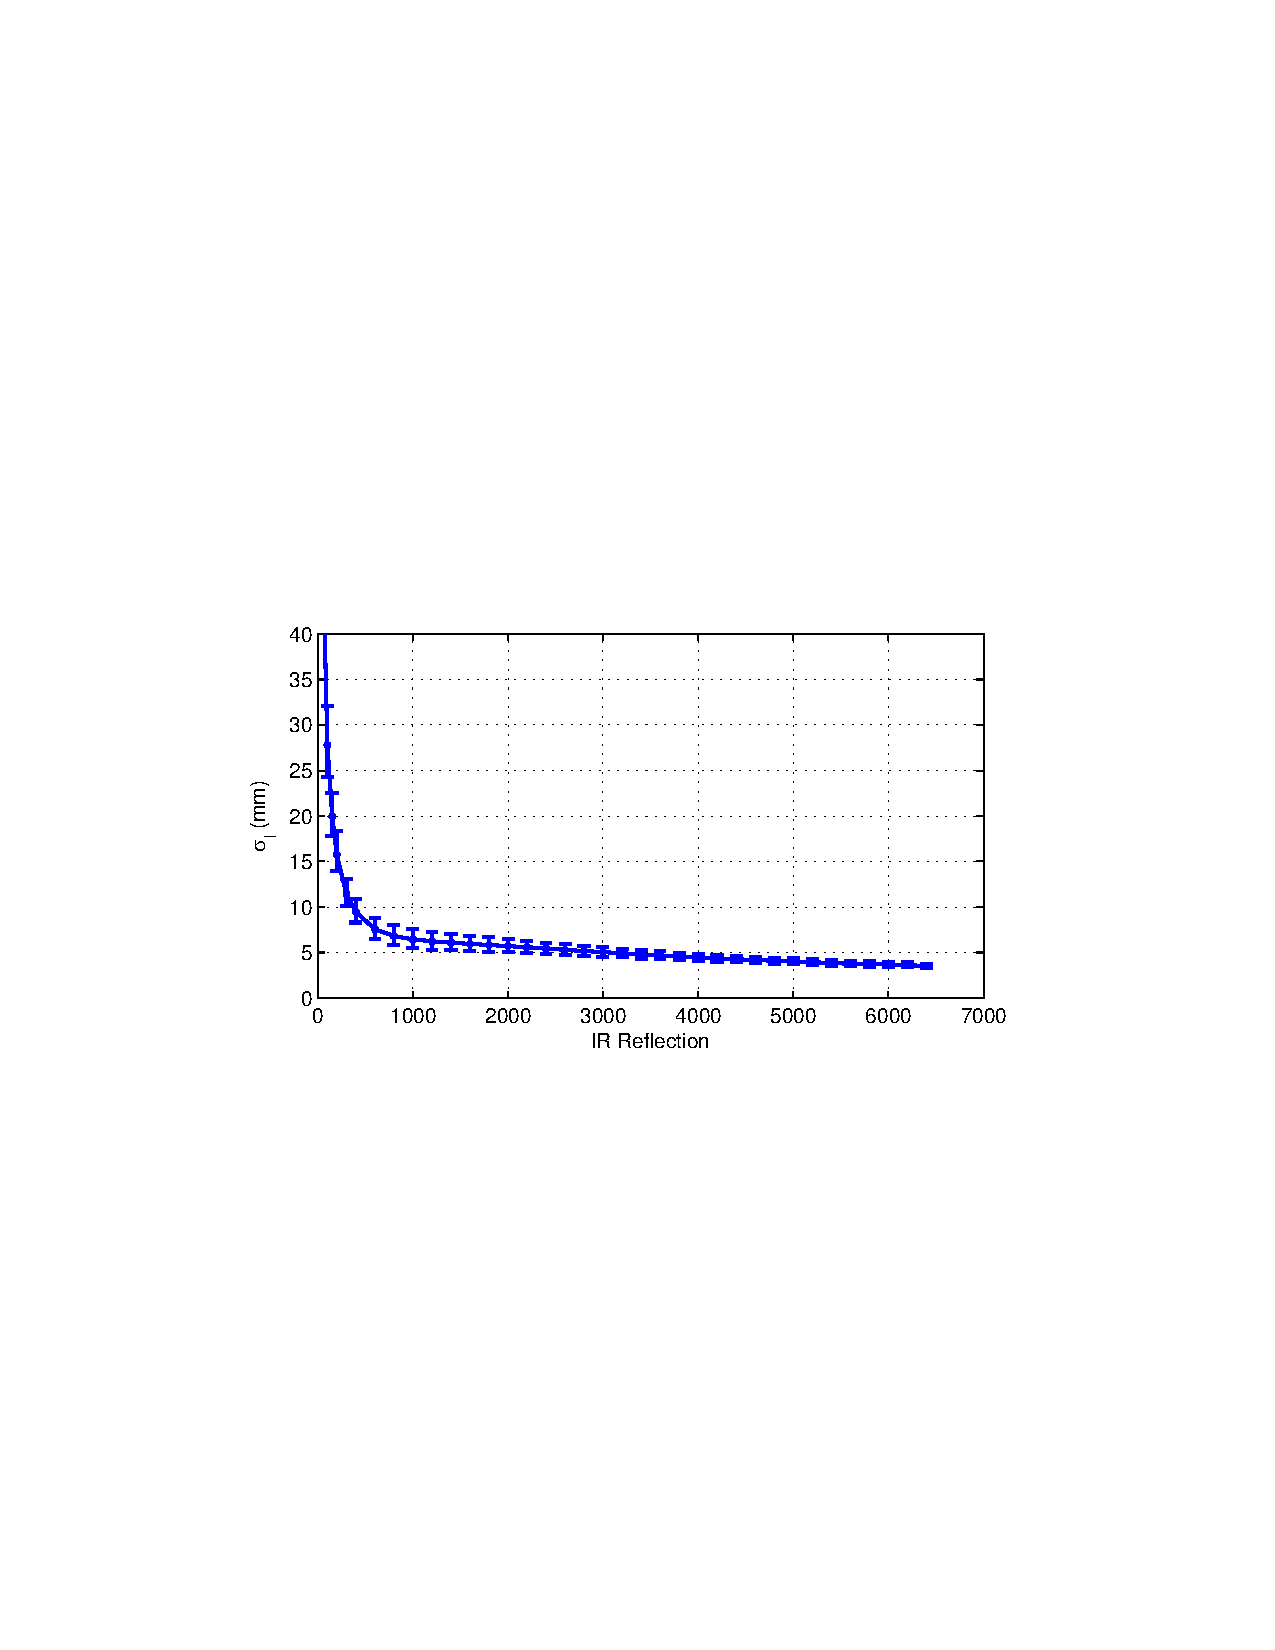
\includegraphics[trim=120 280 110 290,clip,width=0.9\linewidth]{Figures/SigmaInterframe}
\end{center}
   \caption{Image-varying noise, $\sigma_I$, is predicted well by the IR reflectance in raw units returned by the camera, see Figure~\ref{fig:plantnoise}($b$).  The scene-varying noise, $\sigma_S$, is plotted for comparison.}
\label{fig:sigmainterframe}
\end{figure}

Averaging depth measurements of a fixed scene will reduce the noise from $\varepsilon_I$, but will not reduce the noise from $\varepsilon_S$.  This latter scene-varying term is constant for a static scene, but changes when the scene changes.  To characterize this noise we first eliminated (approximately) the image-varying noise contribution by averaging over a large number of images (300).  Then assuming $\varepsilon_S$ is independent and identically distributed between pixels, we measured the variance of the pixel depth errors between a known flat surface and the estimated surface.  In our experiments we obtained $\sigma_S=6.5mm$, and found that it was insensitive to changes in depth.

The total pixel noise can be estimated assuming independence of $\varepsilon_I$ and $\varepsilon_S$, and is given by:
\begin{equation}
\sigma^2 = \frac{\sigma_I^2}{N} + \sigma_S^2,\label{eq:sigma}
\end{equation}
where $N$ is the number of images averaged over.  When averaging 5 or more depth images the scene-varying contribution, $\sigma_S^2$, will dominate.  There are additional sources of noise not modeled by this.  These include object specularities, and mixed-depth pixels on object edges.  These tend to produce very large image-varying noise, $\sigma_I$, and we can filter these points by discarding depth pixels with $\sigma_I>20$mm.  



